\documentclass{projetofinal-dcc}
%%%%%%%%%%%%%%%%%%%%%%%%%%%%%%%%%%%%%%%%%%%%%%%%%%%%%%%%%%%%
%P A C O T E S
%%%%%%%%%%%%%%%%%%%%%%%%%%%%%%%%%%%%%%%%%%%%%%%%%%%%%%%%%%%%
% Adicione aqui seus pacotes

\usepackage{minted}
\usepackage[export]{adjustbox}
\usepackage{float}
\usepackage{url}
\usepackage[utf8]{inputenc}


%%%%%%%%%%%%%%%%%%%%%%%%%%%%%%%%%%%%%%%%%%%%%%%%%%%%%%%%%%%%
%I N I C I O  D O  D O C U M E N T O
%%%%%%%%%%%%%%%%%%%%%%%%%%%%%%%%%%%%%%%%%%%%%%%%%%%%%%%%%%%%
\begin{document}

% título da tese é obrigatório
\title{Automatização de Processos com Redmine e Activiti BPM}

% autor é obrigatório; máximo de 3 autores
\author{Filipe Xavier Trindade dos Santos }{[Aqui entram os agradecimentos]}
\author{Lucas Simões de Sousa Arnaud }{[Aqui entram os agradecimentos]}
\author{Thales Teixeira Pires}{[Aqui entram os agradecimentos]}

% orientador é obrigatório
\advisor[Profª.]{Silvana Rosseto,~Ph.D.}{}

% co-orientador é opcional
%\coadvisor[Prof.]{Nome do co-orientador,~M.Sc.}{}

% máximo de 3 integrantes da banca (orientador e co-orientador já são adicionados automaticamente)
\banca[Prof.]{Nome do participante banca 1,~D.Sc.}{COPPE~-~UFRJ}
\banca[Prof.]{Nome do participante banca 2,~Ph.D.}{COPPE~-~UFRJ}
%\banca[Prof.]{Nome do participante banca 3,~Ph.D.}{COPPE~-~UFRJ}

\location{Rio~de~Janeiro}{RJ}{Brasil}

% mês e ano de defesa
\date{agosto}{2016} %"agosto a gente consegue (by arnaud)
\maketitle

\startdocument

% Sumário 
\maketocpage

%%%%%%%%%%%%%%%%%%%%%%%%%%%%%%%%%%%%%%%%%%%%%%%%%%%%%%%%%%%%
%A G R A D E C I M E N T O S
%%%%%%%%%%%%%%%%%%%%%%%%%%%%%%%%%%%%%%%%%%%%%%%%%%%%%%%%%%%% 
\makethankspage

%%%%%%%%%%%%%%%%%%%%%%%%%%%%%%%%%%%%%%%%%%%%%%%%%%%%%%%%%%%%
%R E S U M O
%%%%%%%%%%%%%%%%%%%%%%%%%%%%%%%%%%%%%%%%%%%%%%%%%%%%%%%%%%%%
\begin{abstract}{
  A eficiência de uma empresa está diretamente relacionada à forma como são conduzidos os seus processos internos. Quanto maior o tamanho da organização, mais importante se torna a sua capacidade de gestão para garantir que eles sejam executados com correção e dentro dos prazos esperados. Uma abordagem efetiva para atingir a eficiência organizacional é a automatização de processos de negócio.

O objetivo deste trabalho é apresentar duas diferentes tecnologias já existentes utilizadas para automatização de processos, o Redmine e os chamados BPMS, e suas principais características, e propor uma forma de integração entre elas, aproveitando as qualidades de ambas para oferecer maior qualidade de gestão, padronização e otimização de recursos na execução de processos de negócio.
}
\end{abstract}

%%%%%%%%%%%%%%%%%%%%%%%%%%%%%%%%%%%%%%%%%%%%%%%%%%%%%%%%%%%%
%A B S T R A C T
%%%%%%%%%%%%%%%%%%%%%%%%%%%%%%%%%%%%%%%%%%%%%%%%%%%%%%%%%%%%
\begin{englishabstract}{
  The efficiency of a company is directly related to the way its internal processes are conducted. The larger the size of the organization, the more important its management capacity becomes to ensure that they are executed with correctness and within the expected time frames. An effective approach to achieving organizational efficiency is the automation of business processes.

The objective of this work is to present two different technologies used for automation of processes, Redmine and the so-called BPMS, and their main characteristics, and to propose a way of integration between them, taking advantage of the qualities of both to offer higher management quality, standardization and optimization of resources in the execution of business processes.
}
\end{englishabstract}

%%%%%%%%%%%%%%%%%%%%%%%%%%%%%%%%%%%%%%%%%%%%%%%%%%%%%%%%%%%%
%L I S T A S
%%%%%%%%%%%%%%%%%%%%%%%%%%%%%%%%%%%%%%%%%%%%%%%%%%%%%%%%%%%%
% Figuras
\makefigurespage

% Tabelas
\maketablespage

% Algoritmos
\makelistingspage

% Abreviaturas (devem estar em ordem alfabética)
\makeabrevpage{\item [BPM] Business Process Management
\item [BPMS] Business Process Management System
\item [BPMI] Business Process Management Initiative
\item [BPMN] Business Process Management Notation
\item [XML] Extensible Markup Language
\item [OMG] Object Management Group


}

% Símbolos (devem estar em ordem alfabética)
% \makesymbolspage{\input{elementos-pretextuais/simbolos}}

%%%%%%%%%%%%%%%%%%%%%%%%%%%%%%%%%%%%%%%%%%%%%%%%%%%%%%%%%%%%
%C O N T E Ú D O
%%%%%%%%%%%%%%%%%%%%%%%%%%%%%%%%%%%%%%%%%%%%%%%%%%%%%%%%%%%%
\startcontent
\chapter{Introdução}\label{chp:introducao}

\section{Motivação}\label{sec:introducao-motivacao}
Os processos de negócio consistem numa sequência de atividades e serviços que  encadeados cumprem determinado objetivo ou função na organização em que é desempenhado. A automatização de processos de negócio consiste na aplicação de tecnologia, de forma que uma ou mais atividades de um processo possam ser automatizadas, reduzindo assim a dependência de atuação humana para sua execução.

\section{Objetivos}\label{sec:introducao-objetivo}
O objetivo geral deste trabalho é propor uma solução para automatização de processos complexos que também contam com interação humana, inclusive durante o fluxo destes. Vamos apresentar uma ferramenta que permite a modelagem de fluxos variados, facilita a configuração e implementação, bem como a utilização contínua por usuários com conhecimentos básicos de processo e o acompanhamento deste por um gerente.

\section{Organização do texto}\label{sec:introducao-organizacao_texto}
\chapter{Redmine}\label{chp:redmine}

\section{Introdução}\label{sec:redmine-introducao}
Neste capítulo vamos explicar como o Redmine, uma ferramenta de gerenciamento de projetos foi utilizada para gestão de processos, ilustrando com um exemplo. Vamos apresentar ainda, a capacidade extensiva desta ferramenta através do desenvolvimento de plugins. Por último vamos abordar as limitações do Redmine que nos motivaram a desenvolver algo novo para atingir nosso objetivo em automatização de processos.

\section{Estrutura básica do Redmine}\label{sec:redmine-estrutura_basica}

A estrutura básica de gerenciamento de projetos no Redmine é composta por X principais elementos. São eles:

\subsection{Tarefas}\label{subsection:redmine-estrutura_basica-tarefa}

São as unidades básicas de execução de trabalho dos projetos (\ref{subsection:redmine-estrutura_basica-projeto}). Elas contém os dados relevantes para o seu gerenciamento (e.g, tipo (\ref{subsection:redmine-estrutura_basica-tracker}, situação(\ref{subsection:redmine-estrutura_basica-status}), data de início, data de conclusão, categoria), para a sua execução (e.g, título, descrição) e dados adicionais que podem variar entre os projetos e tipos de tarefa, que são cadastrados como campos personalizados (\ref{subsection:redmine-estrutura_basica-custom_fields}).  

\subsection{Projetos}\label{subsection:redmine-estrutura_basica-projeto}

\subsection{Tipos de tarefa}\label{subsection:redmine-estrutura_basica-tracker}

\subsection{Situação}\label{subsection:redmine-estrutura_basica-status}

\subsection{Papéis de usuários}\label{subsection:redmine-estrutura_basica-role}

\subsection{Campos Customizados}\label{subsection:redmine-estrutura_basica-custom_fields}


\section{Gestão de processos com o Redmine}\label{sec:redmine-gestao_processos}


\section{Como automatizar um processo?}\label{sec:redmine-automatizar_processo}

\section{Plugins}\label{sec:redmine-plugins}
O Redmine foi desenvolvido de forma a ser extensível por meio de plugins. É possível modificar um funcionalidade da ferramenta, ou criar novas funcionalidades sem precisar alterar o código desta. Os plugins são desenvolvidos em Rails, a mesma linguagem de programação do Redmine. 

Para possibilitar extensões de funcionalidades que envolvem enxertar pedaços de código no meio de uma classe ou de uma tela, o Redmine disponibiliza hooks em diversas partes da ferramenta. São tags com um identificador da parte do código em que estão inseridas. E para utilizar este hook basta incluir um hook listener num plugin, e direcionar qual arquivo ou método um determinado hook vai disparar.

\section{Limitações}\label{sec:redmine-limitacoes}


\chapter{Gerenciamento de Processos de Negócios}\label{chp:bpm}

\section{Introdução}\label{sec:bpm-intro}

Neste capítulo introduziremos o conceito de Gerenciamento de Processos de Negócios, e a notação utilizada para modelar processo de forma padronizada. Falaremos, ademais, dos sistemas que permitem a gestão e condução de processos de forma automatizada. Destacaremos as vantagens e desvantagens deste tipo de sistema, e como esta avaliação contribuiu para a construção de uma solução para a gestão de processos complexos com bastante interação humana.

\section{BPM}\label{sec:bpm-bpm}
BPM\cite{bpm} é o acrônimo em inglês para \textit{Business Process Management}, ou em português \textit{Gerenciamento de Processos de Negócio}. De acordo com van der Aalst\cite{bpm_van_der_aalst}, o BPM é definido como "suporte para processos de negócio, utilizando métodos, técnicas e softwares para projetar, legitimar, controlar e analisar processos operacionais envolvendo humanos, organizações, aplicações, documentos e outras fontes de informação”.

Um processo de negócio é definido por um conjunto de atividades coordenadas, relacionadas entre si, que envolvem diferentes pessoas, procedimentos, áreas e tecnologias com o objetivo de gerar valor para a empresa, seja em forma de produtos ou serviços, internos ou externos.

Diferentemente de métodos tradicionais, que são focados no desempenho das unidades funcionais de uma empresa, a adoção do BPM como disciplina de gestão concentra-se no controle e melhoria contínua dos processos funcionais que, na maioria das vezes, permeiam diferentes áreas de negócio.

A aplicação do BPM não deve necessariamente envolver sistemas. Na prática, diversas melhorias de processos podem ser alcançadas sem a utilização de tecnologia ou sistemas de informação. Por exemplo, através da análise e mapeamento de processos de logística, muitas vezes é possível implementar melhorias no processo através do sequenciamento otimizado das tarefas que o constituem, implicando em menos tempo despendido para sua execução.

Entretanto, quando avaliamos a aplicação de BPM em processos críticos, complexos ou até mesmo processos simples mas executados em maior escala, a aplicação de tecnologia torna-se fundamental. A melhoria e automatização de processos através da aplicação de tecnologia é comumente vista na utilização de sistemas de informação para suportar a execução de diferentes tipos de processos, como ocorre normalmente em um CSC\cite{csc} (Centro de Serviços Compartilhados).


\section{BPMN}\label{sec:bpm-bpmn}
BPMN\cite{bpmn} é o acrônimo em inglês para \textit{Business Process Management Notation}, ou em português \textit{Notação de Gerenciamento de Processos de Negócio}. Foi criada para representar processos de negócio em forma de diagrama, através de uma notação padronizada e de fácil entendimento por diferentes profissionais, sejam eles desenvolvedores, analistas de negócio ou gestores. Foi criada inicialmente pelo BPMI\cite{bpmi} (Business Process Management Initiative) em 2004, entretanto é mantida atualmente pela OMG\cite{omg} (Object Management Group). Sua versão mais atual é a BPMN 2.0\cite{bpmn20}, publicada em 2011.

A notação foi concebida sob a perspectiva de cobrir a falta de entendimento entre diferentes departamentos e organizações a cerca de um determinado processo ou conjunto de processos, algo muito frequente no ambiente corporativo. Além disso, através de sua notação padronizada em XML\cite{xml} (Extensible Markup Language), diferentes ferramentas podem fazer uso de meta-dados para informatizar a orquestração de processos de negócio.



\begin{figure}[H]
  \centering
  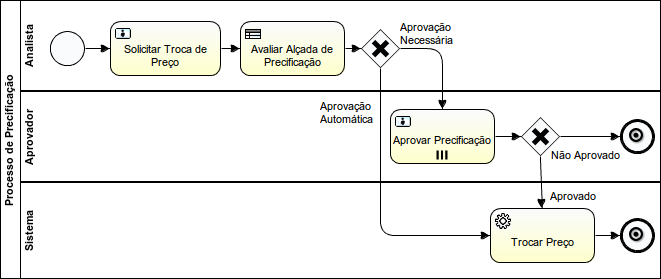
\includegraphics[width=1.0\textwidth]{imagens/ProcessoDePrecificacao.png}
  \caption{Processo representado em BPMN}
  \label{fig:exemplo_bpmn}
\end{figure}

A Figura \ref{fig:exemplo_bpmn} mostra um exemplo de processo modelado na ferramenta Activiti Designer que será abordada em mais detalhes na seção \ref{sec:activiti} e representa o cenário descrito na seção \ref{sec:introducao-caso_real}. Os elementos do modelo serão explicados ao longo deste capítulo.


\subsection{Objetos}\label{sec:bpm-bpmn_objetos}

A notação define quatro grupos distintos de objetos para permitir a diagramação de um fluxo de negócio. Os objetos são classificados em objetos de fluxo, artefatos, agrupadores e conectores. São utilizadas figuras geométricas, como retângulos e círculos, além de linhas pontilhadas e tracejadas, entre outros elementos gráficos para representar cada um dos objetos que constituem a notação.

\subsubsection{Objetos de fluxo}\label{sec:bpm-bpmn_objetos_fluxo}

Os objetos de fluxo são os principais elementos do BPMN pois constituem os elementos chave na execução do fluxo de trabalho. Eles são dividos em 3 principais grupos que serão detalhados a seguir: eventos, atividades e decisões.


\begin{enumerate}
    \item Eventos
    
    Objetos utilizados para representar que algo aconteceu durante a execução do fluxo. São exemplos de eventos: "chamada de sistema externo recebida", "envio de cancelamento do processo recebido", "a cada 1 minuto". A notação BPMN 2.0 define mais de 60 tipos distintos de eventos. A Figura \ref{fig:bpmn_events} mostra alguns dos diferentes tipos de eventos e suas notações.
    
    \begin{figure}[H]
    \centering
    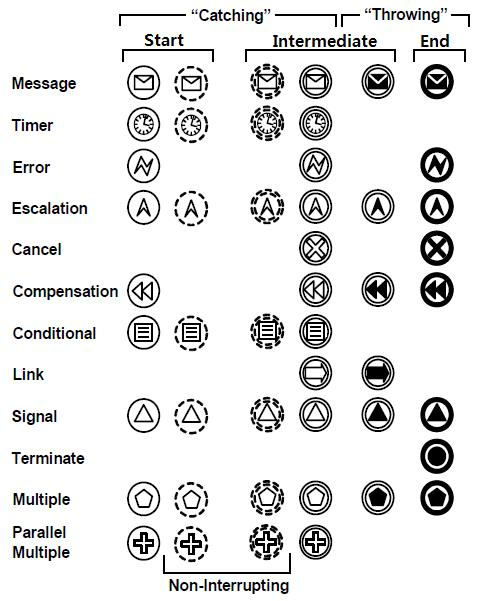
\includegraphics[width=0.65\textwidth]{imagens/bpmn_events.jpg}
    \caption{Tipos de Eventos\cite{tipos_eventos}}
    \label{fig:bpmn_events}
    \end{figure}
    
    Na dimensão horizontal da Figura \ref{fig:bpmn_events}, os eventos estão classificados de acordo com o momento do processo em que podem se manifestar. Os elementos \textit{start} são os eventos que podem criar uma nova instância de processo. Os elementos \textit{intermediate} são os eventos que ocorrem durante a execução do processo. Finalmente, os elementos \textit{end} são os  eventos que indicam o fim do processo, seja por sucesso ou erro.
    
    Na dimensão vertical da Figura \ref{fig:bpmn_events}, os eventos estão classificados de acordo com seu tipo, conforme descrito a seguir:
    \begin{itemize}
      \item  Os eventos \textit{message} são utilizados para indicar um ponto do processo em que ocorre comunicação com um agente externo ou outro processo.
      \item Os eventos \textit{timer} são utilizados para indicar que o processo deverá parar naquele ponto e aguardar até que a condição de tempo parametrizada se torne verdadeira, como por exemplo, uma data específica ou um período de tempo.
      \item Os eventos \textit{error} são utilizados para indicar que ocorreu um erro durante o fluxo de execução do processo. 
      \item Os eventos \textit{escalation} são utilizados para indicar que um outro participante do processo deve executar determinada ação para que o processo continue seu fluxo.
      \item Os eventos \textit{cancel} indicam que o processo e suas atividades devem ser canceladas.
       \item Os eventos \textit{compensation} são utilizados para desfazer ações que já haviam sido completadas e não são mais desejadas e necessitam ser revertidas.
       \item Os eventos \textit{conditional} são utilizados para pausar o processo, até que uma determinada regra de negócio se torne verdadeira.
       \item Os eventos \textit{link} representam uma conexão entre pontos distantes do processo, sendo bastante utilizados em processo com elevado número de atividades para facilitar a visualização do processo. 
      \item Os eventos \textit{signal} são utilizados para comunicação entre processos, porém, diferentemente dos eventos \textit{message} que possuem um destinatário específico, os eventos \textit{signal} executam o modelo \textit{broadcast} para os receptores que dão sequência aos seus fluxos. 
      \item Os eventos \textit{terminate} são utilizados para finalizar completamente a execução de um processo. 
      \item Os eventos \textit{multiple} são utilizados para indicar diversos eventos em um único símbolo com a semântica XOR, ou seja, quando houver ocorrência de qualquer um dos eventos.
      \item Os eventos \textit{parallel multiple} são utilizados para indicar diversos eventos em um único símbolo com a semântica AND, ou seja, somente quando houver ocorrência de todos os eventos.
    \end{itemize}
     
    
    \item Atividades
    
    Objetos utilizados para representar uma unidade de trabalho a ser realizada no processo. Existem dois tipos básicos de atividades: \underline{tarefas} ou \underline{subprocessos}. As tarefas podem ser executadas por humanos ou por algum tipo de serviço, como um seviço web ou mesmo a execução de algum código interno no processo. Já os subprocessos são atividades utilizadas para agrupar outros objetos, encapsulando fluxos de maior complexidade.
    
    \begin{figure}[H]
    \centering
    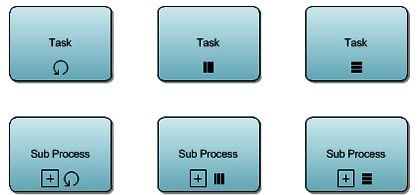
\includegraphics[width=0.55\textwidth]{imagens/bpmn_activities.jpg}
    \caption{Tipos de Atividades\cite{tipos_atividades}}
    \label{fig:bpmn_activities}
    \end{figure}
    
    A mesma atividade pode ser executada uma ou mais vezes, e a Figura \ref{fig:bpmn_activities} mostra as notações utilizadas para indicar multiplicidade. A seta circular nas atividades mais à esquerda indica que estas atividades serão executadas até determinada condição ser satisfeita. Já as linhas paralelas nas outras atividades da figura indicam execuções múltiplas, iterando em cada item de uma coleção previamente definida no processo. As linhas verticais representam que essa iteração ocorre paralelamente, ou seja, cada uma das instâncias da atividade ocorre concomitantemente e sem ordem de execução definida. Já as linhas horizontais significam que a execução das atividades é sequencial, onde uma só será iniciada após o término da anterior.
    
    \item Decisões
    
    São objetos utilizados para controlar o fluxo de trabalho, possibilitando o direcionamento do processo para a escolha de um único sentido, ou para controlar a divergência e convergência de fluxos paralelos. Essas decisões podem ser feitas com base nos dados inerentes ao fluxo do processo ou em eventos relacionados à sua execução.
    
    \begin{figure}[H]
    \centering
    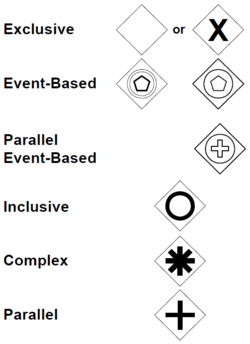
\includegraphics[width=0.4\textwidth]{imagens/bpmn_gateways.png}
    \caption{Tipos de Decisões\cite{tipos_decisoes}}
    \label{fig:bpmn_gateways}
    \end{figure}
\end{enumerate}

    A Figura \ref{fig:bpmn_gateways} mostra a notação dos diferentes tipos de decisões que podem ser aplicadas ao contexto de um projeto. Elas podem ser exclusivas (apenas um fluxo é seguido, notações exibidas na primeira linha), inclusivas (um ou mais fluxos podem ser executados, notação mostrada na quarta linha), complexas (notação que prevê um comportamento específico que envolve uma lógica mais complexa, mostrada na quinta linha), paralelas (todos os fluxos são executados de maneira independente, notação exibida na última linha) e baseadas em eventos, em vez de dados do processo, as quais também podem ser exclusivas (como as notações da segunda linha) ou paralelas (como as notações da terceira linha).


\subsubsection{Agrupadores}\label{sec:bpm-bpmn_objetos_agrupadores}

    São objetos utilizados para organizar visualmente a distribuição dos demais objetos do processo em contêineres que representam a responsabilidade de determinado ator do processo.

    \begin{figure}[H]
    \centering
    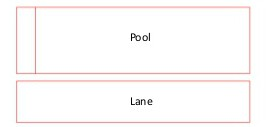
\includegraphics[width=0.5\textwidth]{imagens/bpmn_swimlanes.jpg}
    \caption{Tipos de Agrupadores\cite{tipos_agrupadores}}
    \label{fig:bpmn_swimlanes}
    \end{figure}
    
    A Figura \ref{fig:bpmn_swimlanes} mostra os dois tipos de elementos utilizados para esta finalidade. \textit{Lane} é usada para agrupar tarefas do mesmo usuário, ou grupo de usuários que possuem as mesmas responsabilidades dentro de um processo, já a \textit{pool} é utilizada para agregar diferentes \textit{lanes} do processo. 

\subsubsection{Artefatos}\label{sec:bpm-bpmn_objetos_artefatos}

    São utilizados para acrescentar informações adicionais à modelagem do processo. 

    \begin{figure}[H]
    \centering
    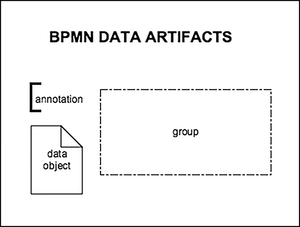
\includegraphics[width=0.5\textwidth]{imagens/bpmn_artifacts.png}
    \caption{Tipos de Artefatos\cite{tipos_artefatos}}
    \label{fig:bpmn_artifacts}
    \end{figure}
    
    A Figura \ref{fig:bpmn_artifacts} exemplifica os diferentes tipos de artefatos. O primeiro são as \underline{anotações}, usadas para adicionar comentários e/ou informações adicionais para facilitar o entendimento do processo, não possui nenhuma influência na execução do fluxo. O segundo é o \underline{objeto de dados} (data object), usado para listar dados inerentes à execução do processo, como um arquivo de entrada, ou um XML\cite{xml} que é gerado como saída de uma etapa e utilizado em outro momento. Estes dados também podem ser variáveis, que serão usadas e manipulados pelos objetos de fluxo, por exemplo, servindo como critério para os objetos de decisão (\ref{sec:bpm-bpmn_objetos}). O terceiro tipo de artefato é o \underline{grupo}, um retângulo utilizado para englobar objetos de fluxo de forma a melhorar a organização do modelo -- assim como as anotações, possui apenas caráter visual, auxiliando a compreensão do processo através de recursos gráficos.


\subsubsection{Conectores}\label{sec:bpm-bpmn_objetos_conectores}

    São utilizados para interligar objetos de fluxo. São classificados em conectores de \underline{sequência}, \underline{mensagem} ou \underline{associação}.

    \begin{figure}[H]
    \centering
    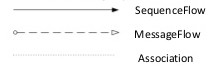
\includegraphics[width=0.5\textwidth]{imagens/bpmn_connectors.jpg}
    \caption{Tipos de Conectores\cite{tipos_conectores}}
    \label{fig:bpmn_conectors}
    \end{figure}
    
    A Figura \ref{fig:bpmn_conectors} mostra a notação utilizada para os três diferentes tipos de conectores. O primeiro é o conector de sequência, que liga os objetos de fluxo, determinando a ordem de execução de cada um deles. O segundo é o conector de mensagem, que indica quando há troca de mensagens entre diferentes atividades, como uma chamada a um serviço \textit{web}, por exemplo. E, por último, a associação simples, que serve para relacionar logicamente diferentes elementos do modelo, mas não altera a execução do fluxo, por exemplo, relacionando um comentário a uma tarefa. 


\section{BPMS}\label{sec:automatizacao-processos-bpms}

BPMS\cite{bpms} é o acrônimo em inglês para \textit{Business Process Management Suites/System}, ou em português \textit{Sistemas de Gerenciamento de Processos de Negócio}. Os softwares BPMS são sistemas especialistas na modelagem, execução, controle e monitoramento de processos de negócio. 

A notação BPMN é utilizada para a modelagem dos processos, e interpretada pelo motor do BPMS que a utiliza para a orquestração do fluxo de trabalho. Devido a sua abordagem focada em processos modelados por uma notação padronizada, o entendimento acerca de um processo de negócio entre analistas de negócio e desenvolvedores acaba sendo facilitado. 

Dentre algumas das vantagens obtidas pelas organizações através da adoção de sistemas BPMS, podemos citar melhorias na capacidade de gestão e monitoramento de processos, melhorias na visibilidade e entendimento de processos, e maior rapidez na introdução de mudanças e ajustes nos processos de negócio.

Dentre alguns aspectos que caracterizam os sistemas BPMS, podemos citar a flexibilidade e facilidade na construção de fluxos de trabalho complexos através de modelagem gráfica, a possibilidade de integração com outros sistemas de informação, os recursos para gestão dos processos e a interface do usuário com as atividades do processo.

Ao inspecionarmos o ecossistema de aplicações BPMS, podemos encontrar diversas opções variando desde soluções caríssimas até soluções gratuitas e de código-fonte aberto. Como exemplo de soluções pagas, podemos citar o SAP NetWeaver BPM\cite{bpm_sap} e Oracle BPM\cite{bpm_oracle}. Como exemplo de soluções com versões gratuitas ou de código-fonte aberto, podemos citar o Activiti BPM\cite{bpm_activiti}, Bonita BPM\cite{bpm_bonita} e Intalio BPM\cite{bpm_intalio}.

A maioria das aplicações BPMS mais robustas oferecem algum tipo de portal para o usuário. Neste portal, o usuário tem a possibilidade de interagir com os processos, atuar em tarefas a ele designadas, iniciar ou finalizar processos, entre outras atividades relacionadas a gestão dos processos. Além do portal, também costumam oferecer algum tipo de API, o que possibilita a utilização de diferentes interfaces com o usuário e integração com outros sistemas. A disponibilidade de uma API permite a extensão e integração do BPMS para outros sistemas, como por exemplo ao permitir a execução de tarefas através de aplicativos em \textit{smartphones}, como na criação de um portal totalmente customizado para atender às necessidades de uma corporação, ou até mesmo na possibilidade de embutir o motor de processos em um sistema para facilitar a orquestração de processos.

Apesar das vantagens e diversos recursos oferecidos por suites BPM, os altos custos deste tipo de solução, além da complexidade para sua implantação e customização de interfaces para o atendimento de diferentes processos, acabam por inviabilizar sua aplicação em projetos corporativos. Neste sentido, buscamos soluções intermediárias, que ofereçam recursos simples e intuitivos para a criação de processos menos complexos, mas que também sejam capazes de escalar para processos mais complexos quando necessário. Além desses aspectos, seria interessante que esta solução não necessitasse da compra de licenças para sua utilização, uma vez que a necessidade de \textit{hardware} e equipe especializada para mapeamento e automatização de processos já incluem custos consideráveis no orçamento de projetos deste tipo.

No próximo capítulo, apresentaremos uma solução desenvolvida neste projeto para atender os requisitos apresentados anteriormente. Um sistema para automatização e gestão de processos, fácil e intuitivo para o usuário, com uma pequena curva de tempo na implantação de processos simples, mas igualmente capaz de suportar processos complexos quando necessário, sem a necessidade de licenças por utilizar \textit{softwares} gratuitos, com uma interface amigável, geração de formulários automáticos, além de uma gestão no controle de acesso a tarefas e processos.
\chapter{Activiti BPM}\label{chp:activiti}

\section{Introdução}\label{sec:activiti-introducao}
Criado em 2010 por ex-integrantes do projeto jBPM, o Activiti BPM é um projeto de código aberto sob a licença Apache V2, que provê um motor BPM leve e completo sob a especificação BPMN 2.0. O Activiti é desenvolvido sob a linguagem de programação Java e é facilmente integrável com aplicações existentes por sua leveza e API amigável.

Neste capítulo vamos apresentar como o Activiti BPM pode ser utilizado na automatização de processos de negócio. Vamos apresentar ainda, a capacidade de modelagem de processos através da notação BPMN utilizada pelo Activiti. Por último vamos abordar as vantagens e limitações desta ferramenta frente às demais opções do mercado.

\section{BPMN}\label{sec:activiti-bpmn}
A BPMN (Business Process Management Notation) foi criada para representar processos de negócio em forma de diagrama, através de uma notação padronizada e de fácil entendimento por diferentes profissionais, sejam desenvolvedores, analistas de negócio ou gestores. Foi criada inicialmente pelo BPMI (Business Process Management Initiative) em 2004, mas atualmente é mantida e atualizada pela OMG (Object Management Group). Sua versão mais atual é a BPMN 2.0, publicada em 2011.

A notação foi concebida sob a perspectiva de cobrir a falta de entendimento entre diferentes departamentos e organizações a cerca de um determinado processo ou conjunto de processos, algo muito frequente no ambiente corporativo. Além disso, através de sua notação padronizada em XML (Extensible Markup Language), diferentes ferramentas podem fazer o uso de sua auto-descrição para orquestração de processos de negócio, sejam eles automatizáveis ou não.

A notação define quatro grupos distintos de objetos para permitir a diagramação de um fluxo de negócio. Os objetos são classificados em artefatos, agrupadores, conectores e objetos de fluxo. São utilizadas figuras geométricas, como retângulos e círculos, além de linhas pontilhadas e tracejadas, entre outros elementos para representar cada um dos objetos que constituem a notação.

1) http://searchcio.techtarget.com/definition/Business-Process-Modeling-Notation

2) http://blog.iprocess.com.br/2012/11/um-guia-para-iniciar-estudos-em-bpmn-i-atividades-e-sequencia

3) https://www.fluig.com/blog/entendendo-melhor-o-bpmn/

\begin{figure}
  \centering
  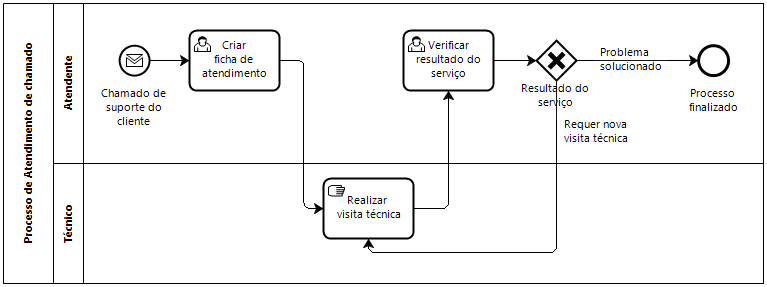
\includegraphics[width=1.0\textwidth]{imagens/bpmn_example.png}
  \caption{Exemplo de processo representado em BPMN}
  \label{fig:exemplo_bpmn}
\end{figure}

\section{Gestão de processos com o Activiti BPM}\label{sec:activiti-gestao_processos}

O motor do Activiti BPM é disponibilizado através de um simples arquivo JAR, modelo de arquivo padrão para bibliotecas da linguaguem Java. Sendo assim, o motor BPM pode ser facilmente utilizado em diferentes projetos Java através da inclusão dessa biblioteca como dependência e pela utilização de sua API.
\section{Como automatizar um processo?}\label{sec:activiti-automatizar_processo}

\section{Vantagens e Limitações}\label{sec:activiti-vantages_limitacoes}



\chapter{Integração Redmine e Activiti BPM}\label{chp:integracao_redmine_activiti}

\section{Introdução}\label{sec:integracao_redmine_activiti-introducao}
Dadas as vantagens e limitações das ferramentas Activiti e Redmine utilizadas como plataformas para a automatização de processos, decidimos desenvolver uma forma de integrá-las para explorarmos os pontos positivos de cada uma delas.

Para atingir este objetivo, criamos um plugin para o Redmine que possibilita a comunicação com o Activiti. Nas próximas sessões, descreveremos o processo de construção deste plugin e como utilizá-lo.


\section{Customização do Redmine}\label{sec:integracao_redmine_activiti-implementacao}

A integração tem por objetivo centralizar o máximo de funcionalidades no Redmine, deixando transparente tanto para o usuário comum como o gestor, a existência de um motor BPM por trás.

\subsection{Funcionalidades}\label{sec:integracao_redmine_activiti_implementacao_funcionalidades}
\subsubsection{Conexão com o Activiti }\label{sec:integracao_redmine_activiti_inplementacao_funcionalidades_conexão}
Para iniciar a utilização do plugin é necessário configurar os detalhes para conexão com o Activiti BPM.
Após colocar o servidor, login e senha, também é preciso disparar os jobs que rodam continuamente para sincronizar os processos e tarefas entre o Redmine e o Activiti.

\subsubsection{Configuração dos estados}\label{sec:integracao_redmine_activiti_inplementacao_funcionalidades_conexão}
Também é necessário configurar os estados principais a serem utilizados pelo plugin.
Configure os estados padrão que devem ser utilizados quando um processo é criado, concluído ou está em andamento.

\subsubsection{Deploy de um processo}\label{sec:integracao_redmine_activiti_inplementacao_funcionalidades_deploy}
Como já foi explicado, o processo deve ser modelado na notação BPMN. Mas à partir deste ponto, toda a interação será através do Redmine.
Na tela de processos, ao clicar em Novo processo, é possível fazer upload de uma modelagem de um processo para o Redmine. Esta operação tenta o deploy do arquivo selecionado no Activiti, através do serviço REST e apresenta o resultado na tela.

A cada vez que esta tela é atualizada, a lista de processos é atualizada. Nela são mostrados todo os fluxos de trabalho ativos no BPMS, inclusive os que não foram instalados através da interface citada acima. Ao clicar numa linha, o usuário consegue visualizar o diagrama do processo.

É possível efetuar o deploy da mesma definição de processo mais de uma vez, caso sejam feitas alterações no fluxo. Neste caso, o novo deploy será identificado como uma nova versão do mesmo processo. 

\subsubsection{Configuração de um processo}\label{sec:integracao_redmine_activiti_inplementacao_funcionalidades_configuracao}
A integração das duas ferramentas se dá na sincronização dos processos e tarefas humanas do Activiti. A representação para elas que foi implementada no Redmine é explicada nas duas seções a seguir:

\begin{itemize}
\item \textbf{Representação de um processo} - Um fluxo de um processo modelado e instalado no Activiti é chamado de definição de processo. No Redmine, o tipo da tarefa representa a definição de processo, e determinará qual o processo que é disparado na criação de uma tarefa. Uma instância (a materialização de uma definição de processo) de um processo no BPMS é iniciada pela criação de uma tarefa no Redmine. Durante toda a vida de um processo, este é representado pela tarefa que deu início a ele. 

\item \textbf{Representação de uma tarefa humana} - Quando um fluxo vai para uma etapa de tarefa humana, é criado uma tarefa no Redmine para representá-la e aonde a interação necessária com o usuário acontecerá. Esta tarefa será filha da tarefa que representa a instância do processo em questão.
\end{itemize}

A primeira configuração a ser feita consiste em definir qual o tipo de tarefa estará conectado ao processo sendo editado. Além disso, é exibida a lista de versões do processo selecionado, e qual a versão ativa. Ao estabelecer esta conexão, toda tarefa deste tipo criada no Redmine disparará uma instância dessa definição de processo no Activiti, na versão ativa marcada.
Na mesma tela também é possível redefinir o nome que aparece na lista de processos.

O próximo passo é editar uma versão para configurar mais detalhes:

\begin{itemize}
\item \textbf{Ativo} - Como explicado anteriormente, ao marcar esta opção, o usuário estabelece a versão padrão que deve ser disparada pelas tarefas conectadas a este processo.

\item \textbf{Variáveis do processo} - Numa definição de um processo podem ser definidas diferentes variáveis a serem usadas para definir o status ou responsável de uma tarefa, para preencher automaticamente um campo ou tomada de decisão. Devem ser preenchidos os valores para essas variáveis utilizadas no processo de acordo com o tipo definido.

\item \textbf{Estados de conclusão do processo} - 
Na modelagem do processo podem ser configurados diferentes eventos de término. Nesta seção são configurados quais status no Redmine vão representar cada evento.

\item \textbf{Configuração das tarefas do processo} - 
Aqui são listadas as etapas do tipo tarefa humana presentes na modelagem. Para cada uma é possível definir o status com o qual deve ser criada cada sub-tarefa que representa a tarefa humana em questão, e definir um tipo de tarefa diferente para cada uma. Caso o campo \textbf{Tipo} não seja preenchido, a sub-tarefa será do mesmo tipo da tarefa original. Caso contrário, a sub-tarefa terá o tipo definido, que pode ser usado para representar um novo processo.

\item \textbf{Campos personalizados utilizados pelo processo} - Na modelagem, o evento de inicialização, bem como as tarefas humanas de um processo possuem campos de formulário. Os valores destes campos são sincronizados junto com as tarefas do Redmine para o Activiti e vice-versa. Para guardar estes campos nas tarefas do Redmine são utilizados campos personalizados. Nesta seção portanto, deve ser selecionado cada campo customizado que representará os campos definidos no processo.

\end{itemize}

\subsection{Detalhes do desenvolvimento}\label{sec:integracao_redmine_activiti_implementacao_detalhes_desenvolvimento}

\subsubsection{Linguagens}\label{sec:integracao_redmine_activiti_implementacao_detalhes_desenvolvimento_linguagens}

O plugin desenvolvido para Redmine foi desenvolvido em Ruby\cite{ruby-lang}, utilizando a framework Rails\cite{rails}. A linguagem open source e orientada a objetos, disponibilizada ao público em 1995, foi criada por Yukihiro “Matz” Matsumoto, inspirada nas linguagens Perl, Smalltalk, Eiffel, Ada e Lisp, suas linguagens preferidas. Em 2006, o Ruby atingiu aceitação massiva, com a formação de grupos de usuários em todas as principais cidades do mundo e com as conferências sobre Ruby com lotação esgotada. Ruby está entre as 10 linguagens mais populares, segundo o índice TIOBE\cite{tiobe} de abril de 2016, que se baseia nas buscas com o nome da linguagem como palavra chave. A framework Rails é uma biblioteca (ou gema) que extende de Ruby. Foi criada por David Heinemeier Hansson em 2004 para a utilização desta linguagem para o desenvolvimento de aplicações web. Isto é feito através da comunicação da comunicação do Ruby com HTML, CSS e Javascript.

As modificações feitas no Activiti foram feitas em Java, a linguagem que em que este foi desenvolvido. Criado em 1995 por um time da Sun (chamado de "Green Team"), Java\cite{java-history} é uma linguagem interpretada orientada a objetos,  que é independente de plataforma, pois sempre executa na JVM (Java Virtual Machine). Segundo o índice TIOBE de abril de 2016 é a linguagem mais popular no mundo.

\subsubsection{Banco de dados}\label{sec:integracao_redmine_activiti_implementacao_detalhes_desenvolvimento_bd}

\subsubsection{Sincronizacao}\label{sec:integracao_redmine_activiti_implementacao_detalhes_desenvolvimento_sincronizacao}

\paragraph{Definição de processo}

% Ao fazer o deploy de um processo através da interface do Redmine é disparado um serviço que acessa a API REST do Activiti, executando uma requisição POST que efetivamente executa o deploy, adicionando a modelagem do processo em questão à lista de definições de processos ativos, que podem ser iniciados.

% O código a seguir monta a requisição POST repository/deployments enviando o arquivo .bpmn, que retorna o deployment\_id do processo cujo deploy acaba de ser feito.

% \codejava{Ruby}{alg:LABEL_CODE_5}{codigos/deploy_process.rb}


% Após executado o serviço é iniciado um job que acessa, através de um outro serviço que busca a definição à partir do deployment\_id. As informações do processo que são recuperadas consistem das tarefas humanas definidas, campos de formulário, variáveis de processo e outros detalhes.

% O código a seguir monta a requisição GET que recupera a definição de um processo.

% \codejava{Ruby}{alg:LABEL_CODE_4}{codigos/process_definition_by_deployment_id.rb}

% O código a seguir consiste do job que centraliza a sincronização de uma definição de processo no momento do deploy. 

% \codejava{Ruby}{alg:LABEL_CODE_3}{codigos/sinchronize_process_definition_job.rb}


\paragraph{Tarefas humanas}\label{sec:integracao_redmine_activiti_implementacao_detalhes_desenvolvimento_sincronizaca_human_task}

\paragraph{Inicialização de um processo}\label{sec:integracao_redmine_activiti_implementacao_detalhes_desenvolvimento_sincronizacao_processo}
% Sempre que uma tarefa é criada, caso ela esteja vinculada a um processo BPM, um serviço é disparado. Este serviço executa 


\subsubsection{Configuracao do processo}\label{sec:integracao_redmine_activiti_implementacao_detalhes_desenvolvimento_configuracao}
% Escrever sobre os detalhes de como modelar um processo que se comunica com o Redmine

\section{Customização do Activiti}\label{sec:integracao_redmine_activiti-implementacao-activiti}

A integração entre o Redmine e o Activiti BPM foi desenvolvida sob o aspecto de direcionar a maior parte das customizações para o lado do Redmine, uma vez que esta é apenas uma das possibilidades de interface com o motor de processos. Num cenário mais amplo de processos mais complexos, outros tipos de dispositivos ou sistemas poderiam realizar uma comunicação direta com os processos.

A API REST padrão oferecida pelo Activiti foi utilizada para a integração entre as ferramentas, uma vez que é bem completa e oferece a maioria dos serviços necessários para a comunicação. Também contou a facilidade de chamadas a APIs REST pelo Ruby on Rails. 

Entretanto, identificamos a ausência de um serviço fundamental para integração entre as ferramentas. Esse serviço deveria retornar uma lista contendo as definições de tarefas contidas em um determinado processo, incluindo os campos disponíveis nos formulários das tarefas. Essa definição nos permitiria estabelecer a interface para o mapeamento dos campos do processo com os campos das tarefas do Redmine.

Sendo assim, extendemos a API REST do Activiti, através da criação de um classe Java representando um novo serviço, semelhante aos serviços existentes no seu código-fonte. Esse serviço consistiu no consumo de uma API Java já disponibilizada pelo Activiti, mas ausente na API REST. O código-fonte simplificado desta classe pode ser observado abaixo:

\codejava{Java}{alg:LABEL_CODE_2}{codigos/TaskDefinitionService.java}

\section{Resultados}\label{sec:integracao_redmine_activiti-resultados}
\chapter{Considerações Finais}\label{chp:conclusao}

\section{Conclusão e Resultados}\label{sec:conclusao-resultados}

O combustível principal deste trabalho, fortemente compartilhado por todos os integrantes, foi a possibilidade de unir o interesse acadêmico e a incrível experiência vivenciada durante todos os anos de estudos na UFRJ com o objetivo de gerar valor para o mercado corporativo através da Visagio\cite{visagio}, empresa na qual trabalhamos há mais de três anos e formada por ex-alunos desta instituição.

Em um cliente da Visagio, onde o Redmine já era utilizado para a gestão de diversos processos na área de Suprimentos, observou-se a necessidade da implantação de fluxos de aprovação mais complexos do que o Redmine poderia oferecer por padrão. Nesse cenário, observamos uma excelente oportunidade para avaliar na prática o funcionamento da solução descrita ao longo deste trabalho.

A figura \ref{fig:process_cartao_compras} demonstra o processo para solicitação de criação de cartão de crédito corporativo. Este processo foi configurado para rodar no Activiti BPM e Redmine, através do \textit{Redmine BPM Integration Plugin} desenvolvido neste trabalho. O processo é disparado mediante a abertura de um chamado no Redmine, onde são preenchidos dados pessoais do solicitante, endereço para entrega do cartão e diretor aprovador. Após a criação do processo, o Activiti BPM imediatamente cria a próxima tarefa: \textit{Workflow Diretor}. Através do mecanismo de sincronização, uma sub-tarefa é criada no Redmine, representando a aprovação do diretor. Esta tarefa tem o responsável definido pelo preenchimento do aprovador na tarefa anterior, sendo encaminhado através do fluxo no Activiti BPM ao Redmine definindo o responsável pela tarefa. Como é possível observar no diagrama, o processo segue por mais dois níveis de aprovação, até finalmente o cartão estar aprovado para emissão e entrega ao solicitante. Caso algum dos aprovadores reprove a solicitação do cartão, o chamado é encerrado e assume o status Reprovado.

\begin{figure}[H]
\centering
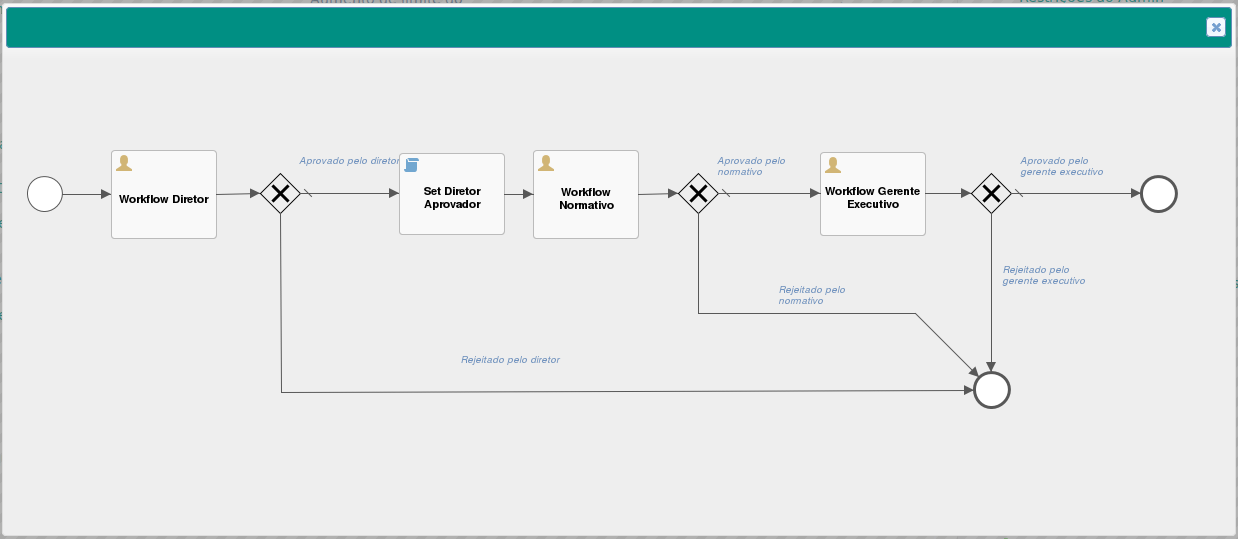
\includegraphics[width=1\textwidth]{imagens/processo_cartao_compras.png}
\caption{Modelo de processo de Criação de cartão corporativo}
\label{fig:process_cartao_compras}
\end{figure}


No caso do processo descrito, a implementação no Activiti BPM permitiu que as tarefas de aprovação fossem atribuídas automaticamente, e que a reprovação de uma etapa resultasse no encerramento do processo com o status Reprovado. Esse comportamento não seria possível de maneira simples no Redmine, diferentemente do Activiti BPM, onde a modelagem permite esse tipo de fluxo de trabalho. O processo descrito anteriormente e outros processos implantados de diferentes complexidades tiveram razão para serem implementados utilizando o plugin desenvolvido, aproveitando-se das facilidades de modelagem e fluxos proporcionados pelo BPM.

No gráfico da figura \ref{fig:grafico_processo} é possível verificar o total de criação e conclusão de três diferentes grupos de processos. Ao observarmos que todos os processos tem um alto percentual de resolução, podemos concluir que a integração entre o Redmine e o Activiti BPM funcionou conforme o esperado, e que os processos fluíram normalmente com a interação dos atores do processo através do Redmine. Além disso, não foram observados reclamações importantes referentes ao funcionamento do fluxo de trabalho. No total, foram iniciados 4.275 processos desde Março de 2016, o que representa uma média de 21 processos iniciados por dia até Setembro de 2016.

\begin{figure}[H]
\centering
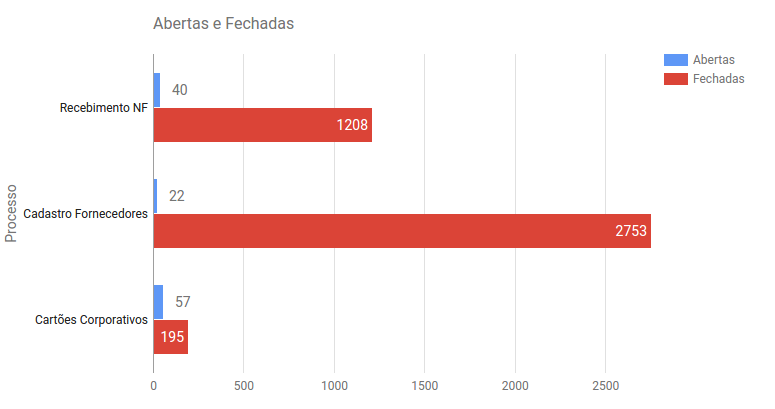
\includegraphics[width=1\textwidth]{imagens/grafico_processo.png}
\caption{Processos utilizando o plugin}
\label{fig:grafico_processo}
\end{figure}


\section{Melhorias Propostas}\label{sec:conclusao-melhorias}

Em alinhamento com a utilização de soluções de código-fonte aberto que compõem este trabalho, todo o código-fonte da integração desenvolvida está disponibilizado no GitHub da Visagio\cite{github_visagio}. O \textit{Redmine BPM Integration Plugin} segue em constante evolução através da implementação desta solução em clientes relevantes no Brasil, o que exige constantes melhorias e avanços no projeto inicial apresentado neste trabalho.

A seguir são apresentadas algumas propostas de melhorias para o seguimento deste trabalho:

\subsection{Tarefas Contínuas}

Durante a implantação, um \textit{feedback} foi recebido pelos usuários do sistema. O plugin introduziu um comportamento um pouco diferente na continuidade do processo do que era de costume no Redmine. Como explicado acima, a representação de uma tarefa humana do Activiti no Redmine é uma sub-tarefa do chamado original que representa o processo. Uma das principais razões desta mudança foi a necessidade de tratar os casos de tarefas humanas que rodam em paralelo, em que no Redmine, cada ator poderia executar sua tarefa isoladamente numa sub-tarefa. 
Esta modificação, no entanto, tirou um pouco a continuidade de um processo em que várias etapas são executadas sequencialmente por um mesmo ator, pois ele não consegue fazer isto apenas avançando as etapas numa mesma tela, mas abrindo cada vez a próxima sub-tarefa que é criada para a próxima etapa. Neste cenário, existe possibilidade de melhorias para melhorar a fluidez quando as tarefas sequenciais são executadas por um mesmo ator.

\subsection{BPMN Integrado}

Neste trabalho utilizamos o Activiti Designer para a modelagem dos processos, que é constituído basicamente do Eclipse com um plugin BPMN. Este cenário apresenta-se pouco prático para usuários sem conhecimento de TI. Nesse sentido, observamos a oportunidade de prover uma modelagem de processos fácil e integrada ao Redmine. Assim, o usuário poderia criar seu processo diretamente na ferramenta, com uma interface simples e online, sem a necessidade de contato com aplicações específicas de desenvolvimento.

Já existem iniciativas similares neste sentido, como o Activiti Modeler\cite{activiti_modeler}, exibido na figura \ref{fig:activiti_modeler}. Portanto, uma melhoria interessante seria acoplar esta ferramenta ao Redmine e avaliar as melhorias necessárias para deixar sua utilização agradável e simples numa única ferramenta.

\begin{figure}[H]
\centering
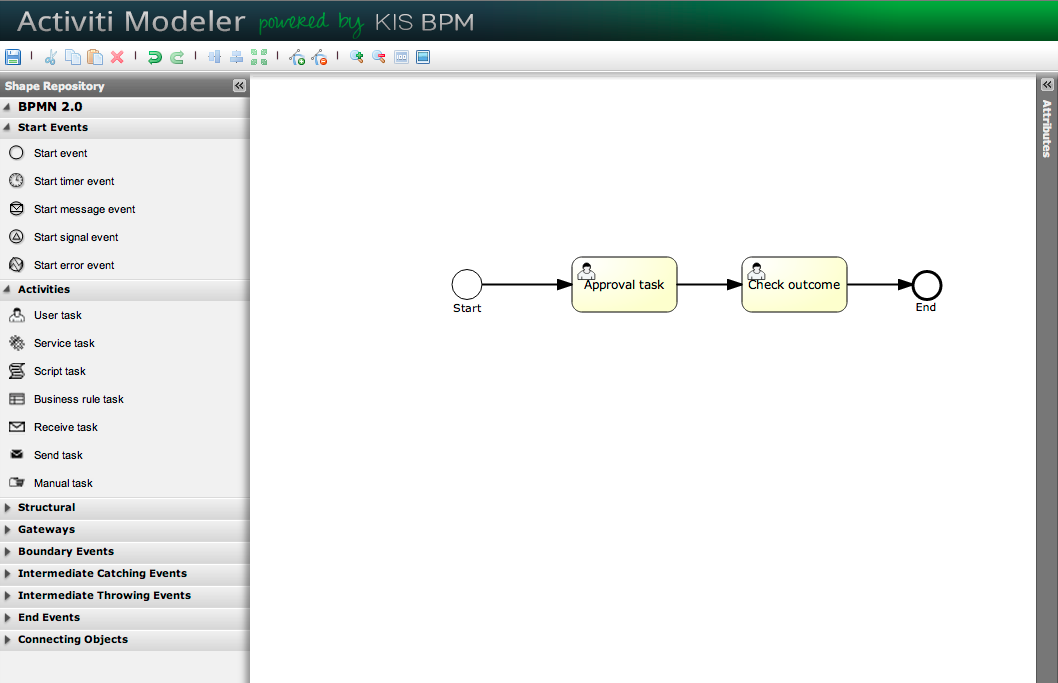
\includegraphics[width=1\textwidth]{imagens/activiti_modeler.png}
\caption{Activiti Modeler}
\label{fig:activiti_modeler}
\end{figure}

\subsection{BRM Integrado}

Uma característica bastante comum em sistemas BPMS é a presença de um BRM (\textit{Business Rules Management}) para gestão de regras de negócio nos processos. O Activiti BPM suporta a integração com o Drools, uma aplicação \textit{web} desenvolvida em Java especialista em BRM. A figura \ref{fig:drools} apresenta uma tabela de decisão no Drools, que pode ser configurada pelo usuário para definir uma regra de negócio baseada em intervalo de valores estabelecendo, por exemplo, a alçada de aprovação em um processo de pagamento.

\begin{figure}[H]
\centering
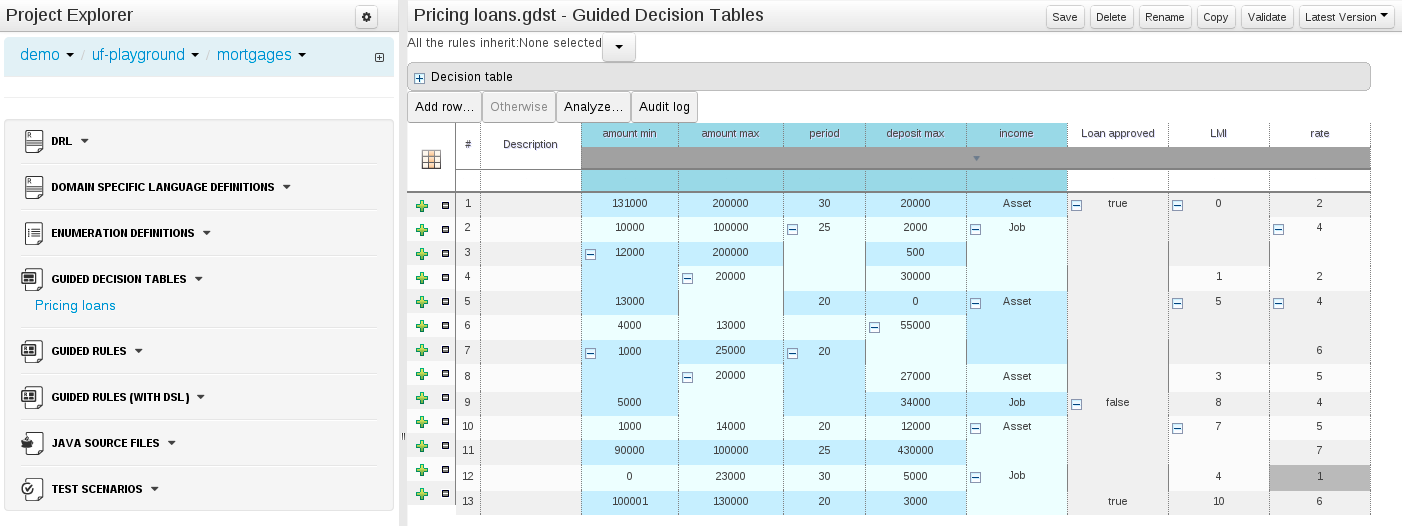
\includegraphics[width=1\textwidth]{imagens/drools_decision_table.png}
\caption{Tabela de decisão no Drools}
\label{fig:drools}
\end{figure}

Uma proposta de evolução no contexto da integração do BPMS com o Redmine, seria o desenvolvimento de plugin BRM, de forma a facilitar a gestão de regras de negócio para processos BPM diretamente no Redmine.

\subsection{BPMS Genérico}

Conforme tentativa apresenta na seção \ref{sec:cenario-integracao-genérica}, esta melhoria proporcionaria uma cadama genérica de integração de qualquer BPMS ao Redmine, flexibilizando assim a escolha do BPMS ou até mesmo a integração com um BPMS que já esteja em uso pela empresa. 
\pagebreak

%%%%%%%%%%%%%%%%%%%%%%%%%%%%%%%%%%%%%%%%%%%%%%%%%%%%%%%%%%%%
% B I B L I O G R A F I A
%%%%%%%%%%%%%%%%%%%%%%%%%%%%%%%%%%%%%%%%%%%%%%%%%%%%%%%%%%%%
% Retirar esta parte se o trabalho não tiver bibliografia
%\bibliographystyle{ieeetr}
%\bibliography{referencias}
\makebibspage{abnt}{elementos-postextuais/referencias}

%%%%%%%%%%%%%%%%%%%%%%%%%%%%%%%%%%%%%%%%%%%%%%%%%%%%%%%%%%%%
% A P E N D I C E
%%%%%%%%%%%%%%%%%%%%%%%%%%%%%%%%%%%%%%%%%%%%%%%%%%%%%%%%%%%%
% Retirar esta parte se o trabalho não tiver anexos
\appendix
\chapter{Processo de Precificação em BPMN}\label{chp:LABEL_APP_1}

    \lstset{
    language=xml,
    tabsize=3,
    %frame=lines,
    caption=Código do Processo de Precificação em BPMN,
    label=code:process_bpmn,
    frame=shadowbox,
    rulesepcolor=\color{gray},
    xleftmargin=20pt,
    framexleftmargin=15pt,
    keywordstyle=\color{blue}\bf,
    commentstyle=\color{OliveGreen},
    stringstyle=\color{red},
    numbers=left,
    numberstyle=\tiny,
    numbersep=5pt,
    breaklines=true,
    showstringspaces=false,
    basicstyle=\footnotesize,
    emphstyle={\color{magenta}}}
    \lstinputlisting{codigos/process.xml}

\chapter{REST de Definições de Tarefas}\label{chp:LABEL_APP_1}

     \lstset{
    language=java,
    tabsize=3,
    %frame=lines,
    caption=REST de Definições de Tarefas,
    label=code:task_definition_service,
    frame=shadowbox,
    rulesepcolor=\color{gray},
    xleftmargin=20pt,
    framexleftmargin=15pt,
    keywordstyle=\color{blue}\bf,
    commentstyle=\color{OliveGreen},
    stringstyle=\color{red},
    numbers=left,
    numberstyle=\tiny,
    numbersep=5pt,
    breaklines=true,
    showstringspaces=false,
    basicstyle=\footnotesize,
    emphstyle={\color{magenta}}}
    \lstinputlisting{codigos/TaskDefinitionService.java}

\end{document}